
\chapter{IMAX3 Software}

\section{IMAX3 interface mapped on CPU memory space}

IMAX3 is just a group of multiple lanes of IMAX2 connected to a
large-capacity external memory. The hardware/software interface of IMAX3 is
a set of control interfaces for each IMAX2.

\section{Dataflow example}

\begin{figure}[htbp]
\center
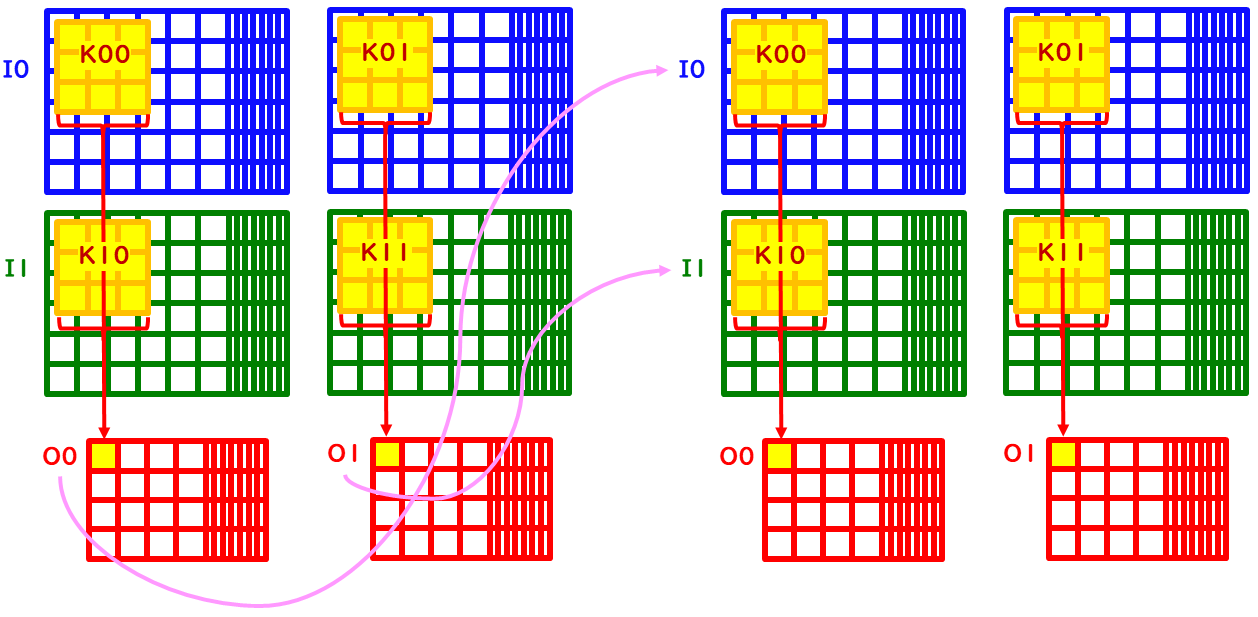
\includegraphics[angle=270,origin=b,width=0.80\textwidth]{fig35.eps}
\caption{\label{fig:4dconv}Tycal series of 4D-array convolution}
\end{figure}

\begin{figure}[htbp]
\center
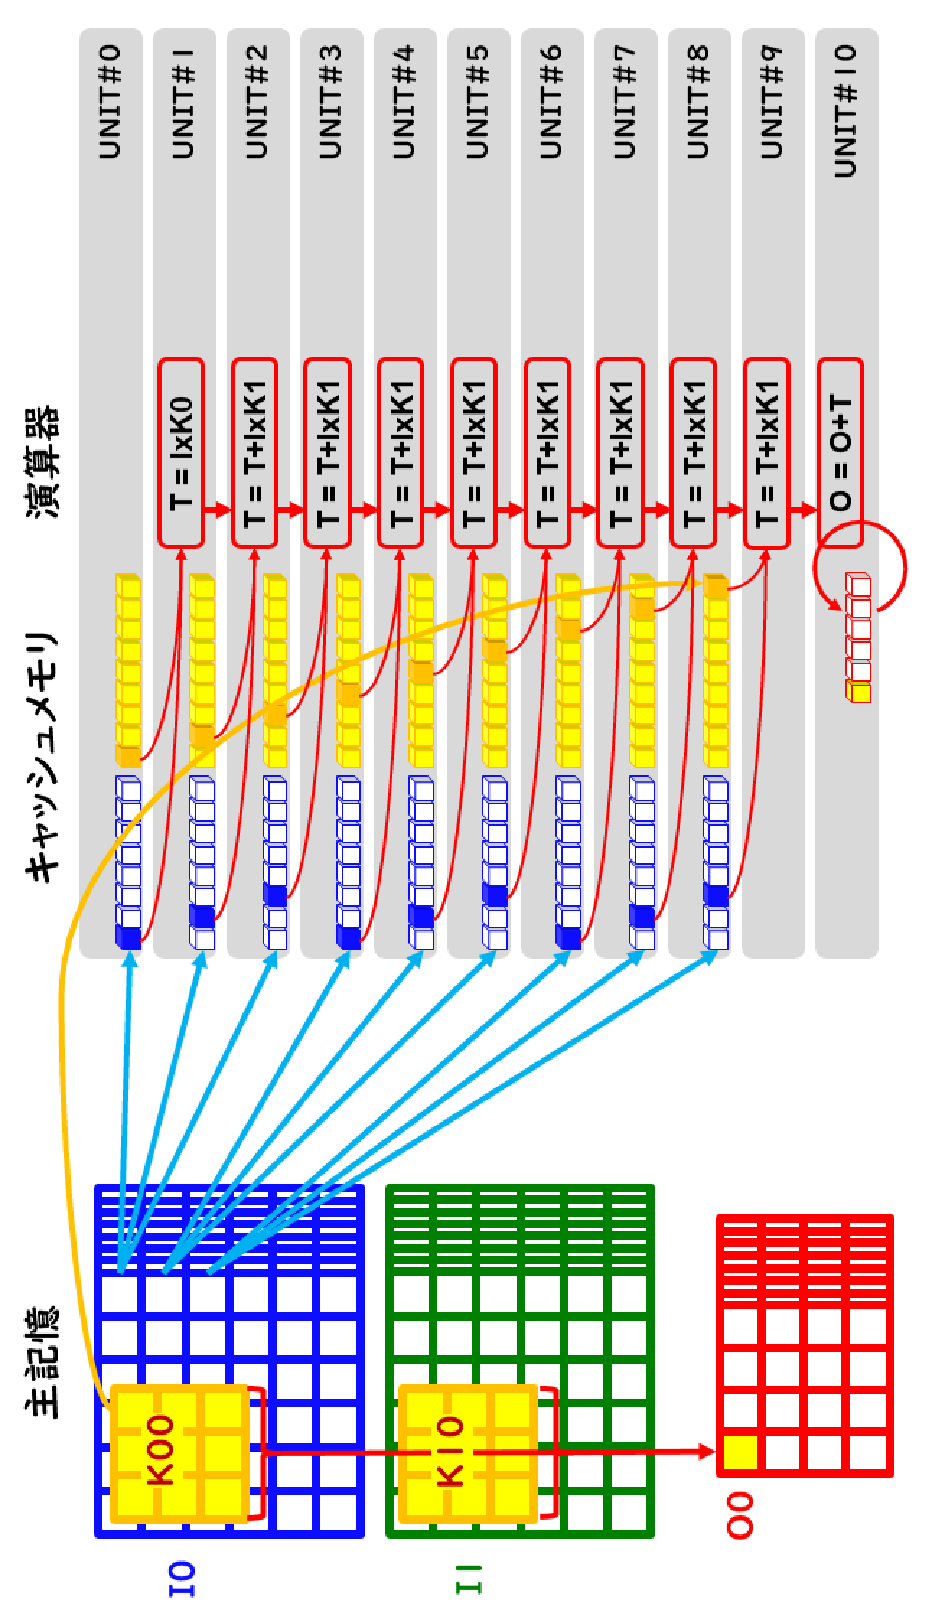
\includegraphics[angle=270,origin=b,width=0.80\textwidth]{fig36.eps}
\caption{\label{fig:4dmap}Typical mappting of convolution}
\end{figure}

\begin{figure}[htbp]
\center
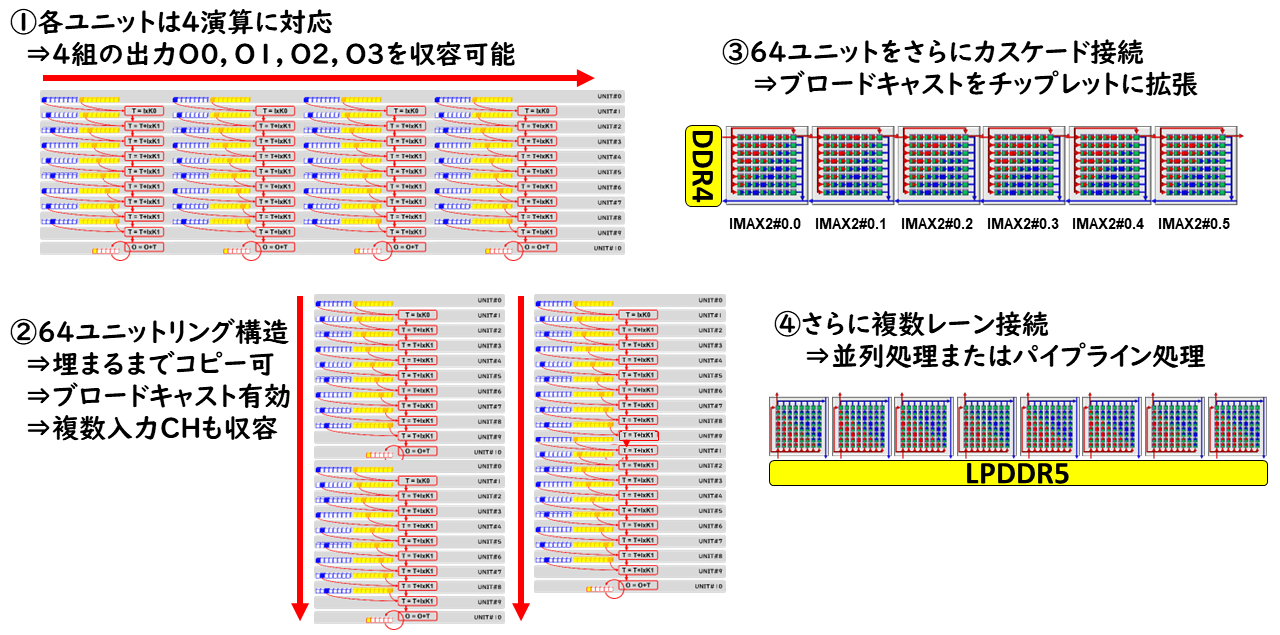
\includegraphics[angle=270,origin=b,width=0.80\textwidth]{fig37.eps}
\caption{\label{fig:options}Several options to speedup convolution}
\end{figure}

\begin{figure}[htbp]
\center
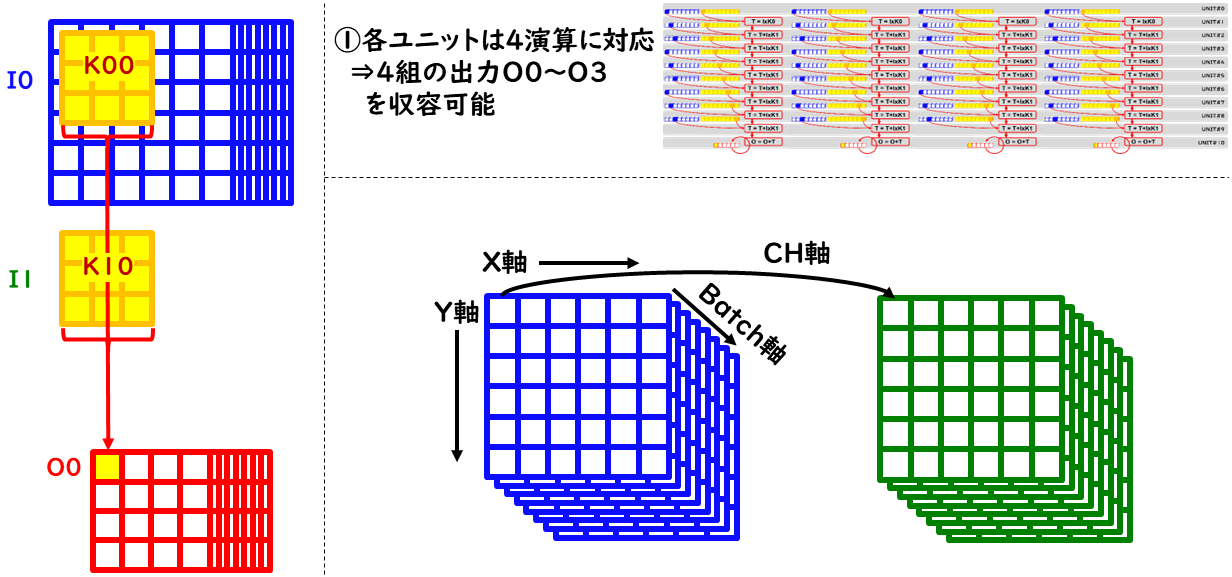
\includegraphics[angle=270,origin=b,width=0.80\textwidth]{fig31.eps}
\caption{\label{fig:twoaxis}Selecting two axis from 4D array}
\end{figure}

\begin{figure}[htbp]
\center
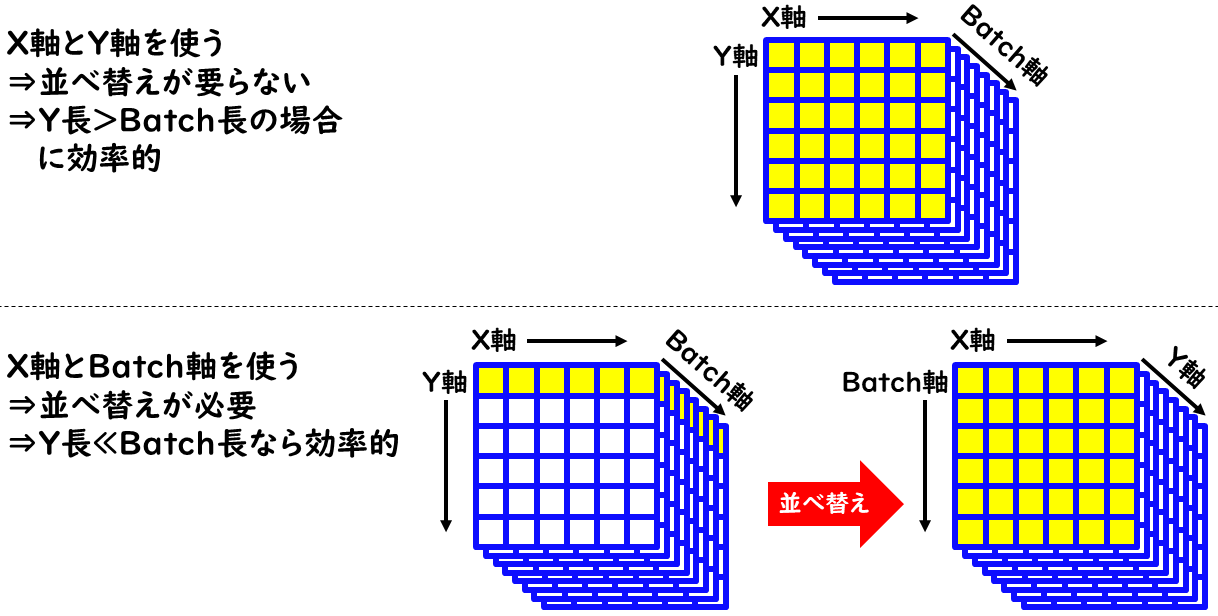
\includegraphics[angle=270,origin=b,width=0.80\textwidth]{fig32.eps}
\caption{\label{fig:optimal}Two options to increase the length of the burst execution}
\end{figure}
 
Figure \ref{fig:4dconv} shows a typical convolution
operation. Multiplication of a part of the input data (I) and the
corresponding kernel (K), and accumulation produce the result. The shape
that 6x6 two-dimensional I0 overlap in the depth direction corresponds to
multiple 6x6 images being included in one batch. I1 has a similar structure.
For example, I0 corresponds to the blue component and I1 corresponds to the
green component. There are many pairs of input data and kernels, and the
vertical summation is the output O0. Since the input data is two-dimensional
and the calculation is repeated by shifting the kernel K in the X and Y
directions, the output O0 is also two-dimensional. Also, if you keep the
input data (I) as is and replace only the kernel (K) and perform the same
calculation, you will find another output O1. In other words, the input data
(I), kernel (K), and output data (O) are all 4-dimensional
arrays. Furthermore, in the multilayer convolution operation, the same
calculation is repeated using the output data (O) as the next input data
(I).

There are several ways to perform the above convolution operations using
IMAX3. Fig.\ref{fig:4dmap} is the basic form of two-dimensional convolution.
Each IMAX unit contains cache memory and a computing unit that are
controlled by the host driver. Blue input data in main memory is broadcast
to the blue part of the cache memory, and yellow kernels in main memory are
broadcast to the yellow part. Unit 0 extracts the data corresponding to the
upper left corner of the kernel and sends it to unit 1. Unit 1 performs the
multiplication and sends the result to unit 2. By connecting the above,
finally, unit 10 accumulates the sum of the 9 multiplication results to the
red output, and completes one 3x3 convolution operation. All units perform
calculations one after another while shifting the input data to the right,
and the output data is updated continuously. The above is a typical CGRA
calculation method.

A feature of IMAX is the large number of degrees of freedom in combining the
above basic shapes according to the size of the 4-dimensional array
(Fig.\ref{fig:options}). The goal of optimization is to reduce execution
time, and the methods are broadcasting and maximum reuse of cache
memory. One chip of IMAX2 can continuously execute double loops at once, and
can map four sets of convolution operations into a logical four-column
structure. What remains is which axis of the 4-dimensional data should be
mapped to the double loop. Once you decide which axis of input I to select,
the others will be determined automatically, so first select the axis of
blue input data (I). There are four candidates: the X axis, Y axis, batch
axis, and channel axis, as shown in Fig.\ref{fig:twoaxis}. However, the
X-axis should be selected because the addresses are continuous. Similarly,
the channel axis is efficient if used to fill 64 units, so the remaining
axes have two choices: the Y axis or the batch axis.

Figure\ref{fig:optimal} shows two mapping methods. When using the X and Y
axes, the yellow data does not need to be reshaped because it is a
continuous address. It is most efficient if the data size of one sheet,
which is the product of the length of X and the length of Y, is stored in
the cache memory within the unit. For example, if the cache memory is
16Kwords, it can accommodate up to 128x128. In the case of 256x256, you can
keep this format and divide it into four in the Y direction. On the other
hand, after multilayer convolution, the result is a small square such as
2x2, which shortens IMAX's continuous execution time and increases startup
overhead. In such cases, use the batch axis instead of the Y axis. Although
the overhead associated with reshaping increases, if the number of batches
is 100, it becomes 2x100, which allows the data size to be increased and the
startup overhead to be reduced. In the case of 3D convolution, you can
similarly increase the continuous operation time of IMAX and reduce the
number of startups.

\section{Programming model of Macro pipelining}

\begin{figure}[htbp]
\center
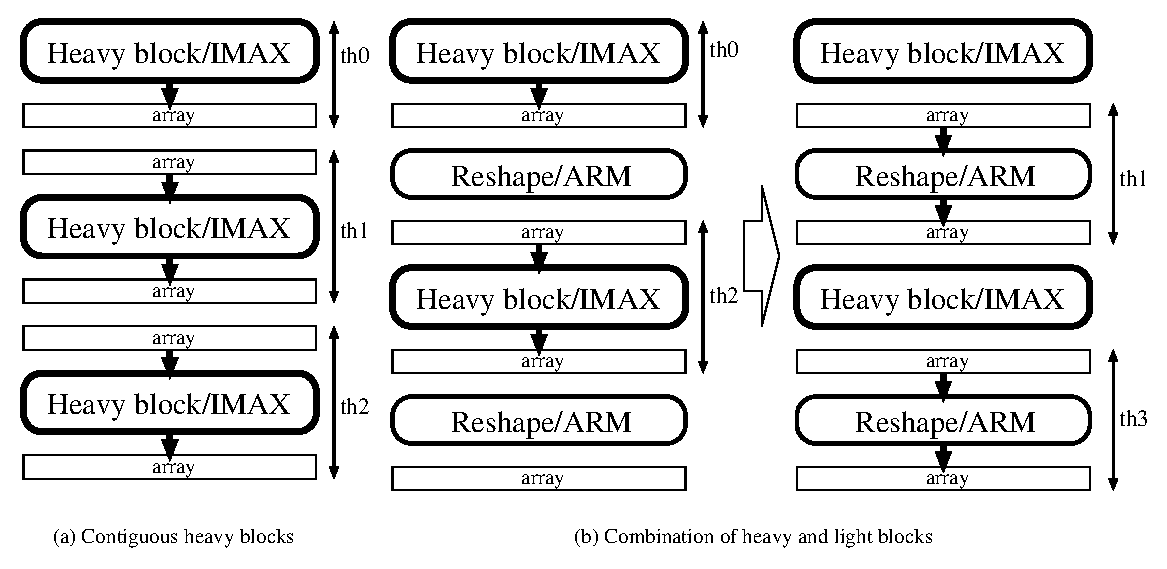
\includegraphics[angle=0,origin=b,width=0.85\textwidth]{macro-pipe.eps}
\caption{\label{fig:model0}Programming model}
\end{figure}

Figure\ref{fig:model0} is the programming model related to macro pipelining. 
In (a), there are three sections with long processing times, and the macro
pipelining is performed. The main thread starts three threads and speeds up
each section using IMAX. A double buffer is required for the data structure
between threads so that the input and output of each thread do not
interfere. On the other hand, (b) is a case where the long processing time
is executed by IMAX, but there is short-term processing by the host, such as
exchanging array indexes, between the heavy processing. By using short-time
processing as a double buffer, memory usage can be reduced compared to
applying double buffers between all threads.

\section{Programming style of Macro pipelining}

\begin{figure}[htbp]
\center
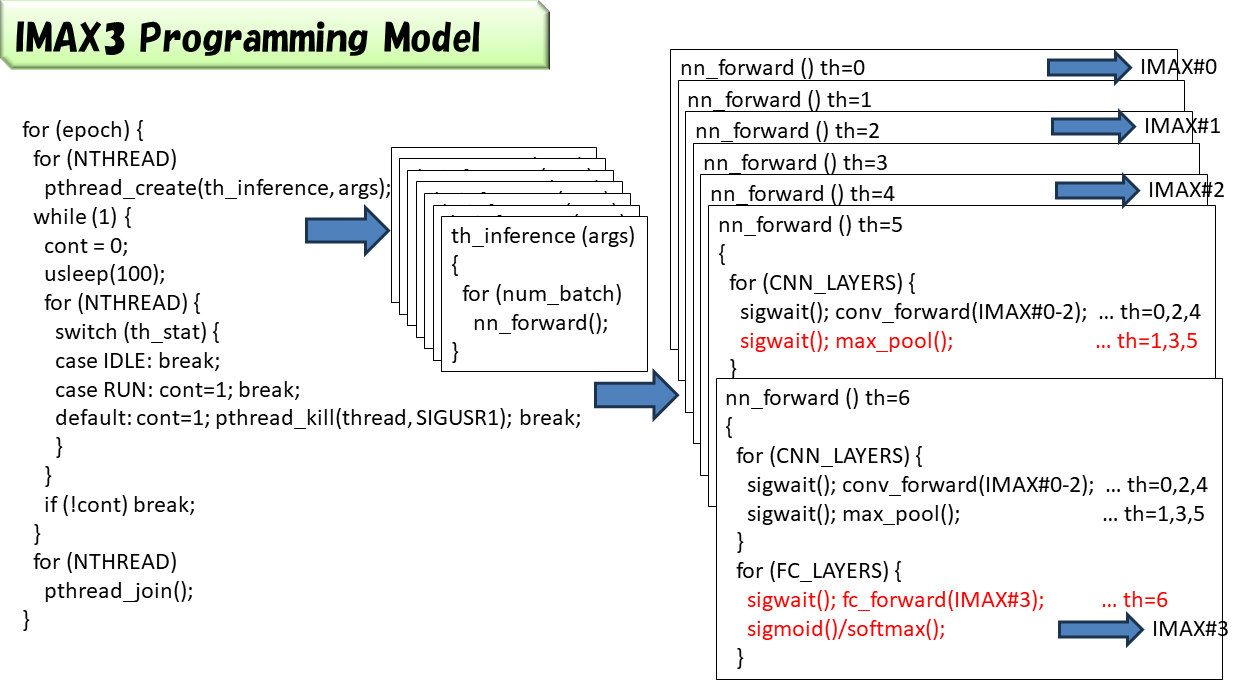
\includegraphics[angle=270,origin=b,width=0.85\textwidth]{fig15.eps}
\caption{\label{fig:model1}Programming style}
\end{figure}

Figure\ref{fig:model1} is the programming style. For the macro pipelining,
multiple threads are started, and the function (th\_inference) containing
the loop structure is executed in parallel. The th\_inference() repeatedly
executes nn\_forward(), which simulates a multilayer CNN. Although
nn\_forward() is executed simultaneously by multiple threads, each thread
executes only the part it is responsible for, and performs pipeline
processing while waiting to complete processing in the previous and
subsequent layers. In each layer, function calls that take LANE as an
argument use IMAX2. Multiple HOSTs and IMAX2 participate in macro
pipelining.  By using sigwait() instead of a busy loops, waiting between
threads can be performed on HOST even if HOST does not have enough cores.
